\thispagestyle{hoccungpinone}
\pagestyle{hoccungpi}
\everymath{\color{hoccungpi}}
\graphicspath{{../hoccungpi/pic/}}
\blfootnote{$^{1}$\color[named]{hoccungpi}Hà Nội.}
\begingroup
\AddToShipoutPicture*{\put(0,616){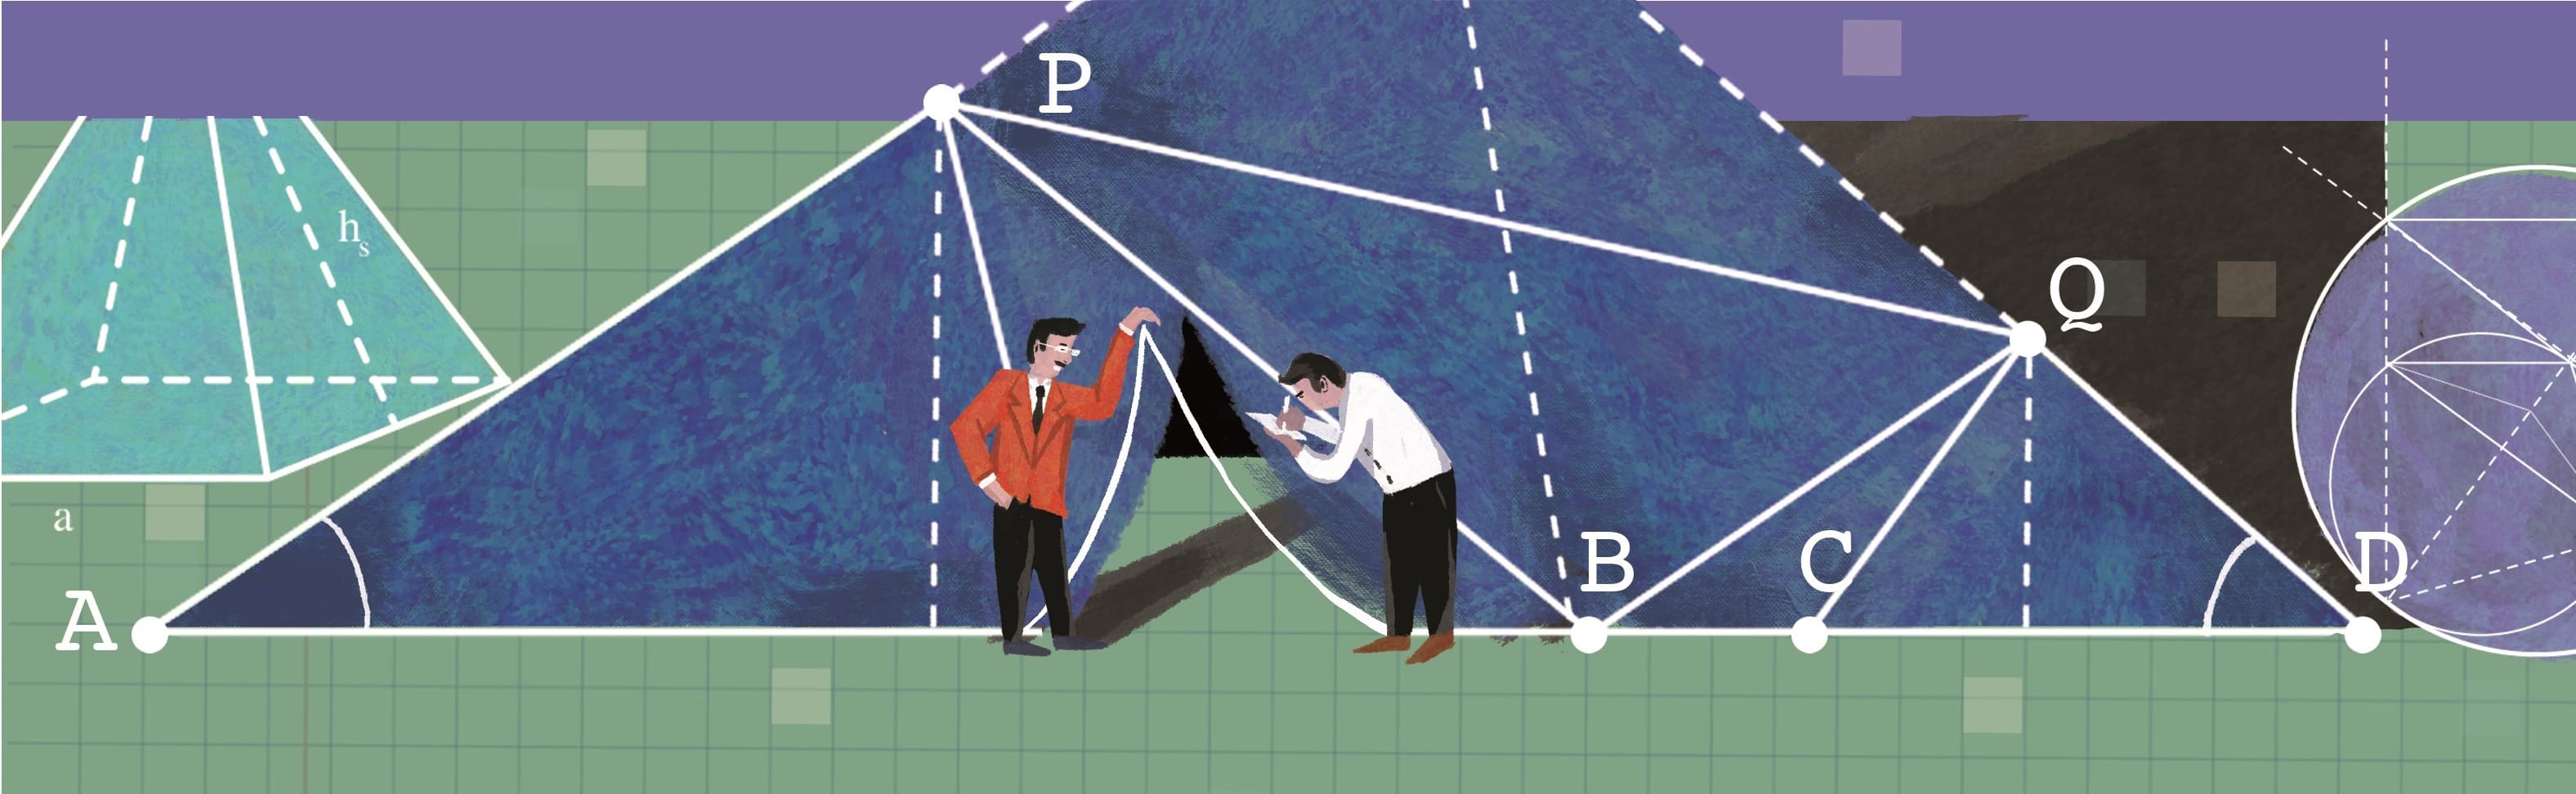
\includegraphics[width=19.3cm]{../bannerhoccungpi}}}
\AddToShipoutPicture*{\put(90,523){
\includegraphics[scale=1]{../tieude.pdf}}}
\centering
\endgroup
\vspace*{185pt}

\begin{multicols}{2}
	Bài toán hai cái can là một loại bài toán rất quen thuộc ở bậc tiểu học. Trong đó, ta cần tìm cách để sử dụng hai cái can với dung tích $a$ và $b$ lít để đong được $k$ lít nước từ bể. Trong bài viết này, chúng ta hãy tìm hiểu mối liên hệ giữa bài toán trên và lý thuyết số.
	\vskip 0.1cm
	$\pmb{1.}$ \textbf{\color{hoccungpi}Bổ đề Bézout và vấn đề tồn tại nghiệm}
	\vskip 0.1cm
	Trong lời giải của bài toán hai cái can nêu trên, ta có những loại thao tác sau:
	\vskip 0.1cm
	$\bullet$ Loại $1$: Đổ đầy một can rỗng hoặc đổ hết nước trong một can đầy trở lại bể
	\vskip 0.1cm
	$\bullet$ Loại $2$: Đổ từ một can đầy sang can rỗng
	\vskip 0.1cm
	$\bullet$ Loại $3$: Đổ toàn bộ nước trong một can (không đầy) sang can rỗng còn lại
	\vskip 0.1cm
	$\bullet$ Loại $4$: Đổ từ một can đầy sang một can đã có một lượng nước nhất định. 
	\vskip 0.1cm
	Trong các loại thao tác trên, lượng nước trong các can sau các thao tác loại $1$ hoặc $2$ đều có thể  biểu diễn bởi các số $a$, $b$ hoặc hiệu của chúng. Thao tác loại $3$ chỉ chuyển vị trí lượng nước. Thao tác loại $4$ bắt đầu từ một trạng thái sau một thao tác loại $4$ khác hoặc từ lượng nước sau một thao tác loại $2$. Do đó, lượng nước ở các can sau thao tác loại $4$ cũng có thể được biểu diễn bằng tổng, và hiệu của nhiều số hạng có giá trị $a$ hoặc $b$. Lượng nước cuối cùng mà ta đong được cũng phải thuộc dạng này.
	\vskip 0.1cm
	Nói cách khác, lượng nước cuối cùng mà ta đong được có dạng theo biểu thức: 
	\begin{align*}
		s\cdot a+ t\cdot b
	\end{align*}
	với $s,t$ là các số nguyên (dạng biểu thức này còn được gọi là một tổ hợp tuyến tính của $a$ và $b$). Để trả lời câu hỏi với các giá trị nào của k thì bài toán có nghiệm, chúng ta sẽ sử dụng bổ đề Bézout trong lý thuyết số.
	\begin{figure}[H]
		\centering
		\vspace*{-5pt}
		\captionsetup{labelformat= empty, justification=centering}
		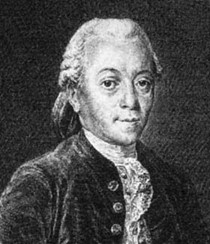
\includegraphics[width=0.75\linewidth]{1}
		\caption{\small\textit{\color{hoccungpi}Étienne Bézout $(1730 - 1783)$.}}
		\vspace*{-10pt}
	\end{figure}
	Bổ đề Bézout (đặt tên theo nhà toán học Pháp, Étienne Bézout ) được phát biểu như sau:
	\vskip 0.1cm
	\textit{Ước chung lớn nhất $d$ của hai số dương $a$ và $b$ luôn có thể được viết dưới dạng $d=s\cdot a+t\cdot b$ với $s,t$ là các số nguyên. Đồng thời, bất kỳ số nguyên nào có dạng $m\cdot a+n\cdot b$ đều là một bội số của $d$.}
	\vskip 0.1cm
	Bổ đề này cho phép ta nhận xét như sau về bài toán hai can nước: với $k$ là số lít nước cần đong, bài toán hai can nước có cách giải khi và chỉ khi $k$ là một bội số của ước chung lớn nhất của $a$ và $b$. Chẳng hạn, với hai can $8$ lít và $12$ lít, do ước chung lớn nhất là $4$ nên ta chỉ có lời giải cho các giá trị cần đong là bội của $4$.
	\vskip 0.1cm 
	Phần sau của bổ đề Bézout có thể được chứng minh một cách dễ dàng từ phần trước. Vì $d$ là ước chung lớn nhất của $a$ và $b$ nên $a=a_0\cdot d$, $b=b_0\cdot d$. Do đó ta luôn có $m\cdot a+n\cdot b=(ma_0+nb_0)\cdot d$.
	\vskip 0.1cm
	Phần trước của bổ đề có một số cách chứng minh khác nhau. Chúng ta hãy cùng tìm hiểu cách chứng minh xuất phát từ thuật toán Euclid. 
	\vskip 0.1cm
	$\pmb{2.}$ \textbf{\color{hoccungpi}Thuật toán Euclid}
	\vskip 0.1cm
	Thuật toán Euclid cho phép chúng ta tìm ước chung lớn nhất của hai số một cách nhanh chóng mà không cần phải tiến hành phân tích ra thừa số nguyên tố. Ban đầu, nó được Euclid phát biểu cho các độ dài đoạn thẳng. Sau đây, chúng ta sẽ mô tả thuật toán này theo ngôn ngữ toán học hiện đại.
	\vskip 0.1cm
	Thuật toán Euclid được xây dựng dựa trên các nhận định sau cho hai số dương $a$ và $b$:
	\vskip 0.1cm
	$\bullet$ $\text{ƯCLN}(a,b) = \text{ƯCLN}(b,a)$					\hfill ($1$)
	\vskip 0.1cm
	$\bullet$ Nếu $a>0$ và $b \,\vdots \,a$ thì $\text{ƯCLN}(a,b) = a$			\hfill ($2$)
	\vskip 0.1cm
	$\bullet$ Nếu $a$ chia cho $b$ dư $c$ thì $\text{ƯCLN}(a,b) = \text{ƯCLN}(c,b)$		\hfill ($3$)
	\vskip 0.1cm
	Hai nhận định đầu tiên ($1$) và ($2$) có thể dễ dàng được chứng minh. Để chứng minh nhận định ($3$), ta sử dụng một số tính chất của phép chia hết. 
	\vskip 0.1cm
	Vì $c$ là số dư trong phép chia cho $b$ nên $a=c+b\cdot y$ với $y$ là một số dương. Gọi $t$ là một ước chung của $b$ và $c$. Do $b\,\vdots\, t$ nên $b\cdot y\, \vdots\,t$. Đồng thời, $c\,\vdots\,t$ nên $a=c+b\cdot y\,\vdots\,t$. Nói cách khác, mọi ước chung của $b$ và $c$ cũng đều là ước chung của $a$ và $b$. 
	\vskip 0.1cm
	Tương tự, khi viết $c=a-b\cdot y$, ta cũng có thể chứng minh mọi ước chung của $a$ và $b$ cũng là ước chung của $b$ và $c$. 
	\vskip 0.1cm
	Do đó, hai tập hợp ước chung này là như nhau nên phần tử lớn nhất của chúng cũng như nhau hay hai cặp số sẽ có chung ước chung lớn nhất.
	\vskip 0.1cm
	Với những nhận định trên, ta có thể tìm ước chung lớn nhất của hai số bằng cách lập một dãy số. Giả sử $a>b$. Đặt $r_0=a,r_1=b$. Sử dụng quy tắc từ ($3$):
	\begin{align*}
		r_{n+1}=r_{n-1}  \mod r_n
	\end{align*}
	(ở đây $\mod$ là toán tử cho ra số dư của phép chia hai số), ta xây dựng được một dãy số giảm dần: $r_0>r_1>r_2>r_3>\cdots$ và do đó sẽ tồn tại một giá trị $N$ sao cho $r_N=0$ (dãy số không thể nhận giá trị âm). Khi đó, $r_{N-2}\,\vdots\,r_{N-1}$. Từ ($2$) và ($3$), ta có $r_{N-1}$ chính là ước chung lớn nhất của hai số ban đầu.
	\vskip 0.1cm
	Ví dụ, với $a=30,b=18$, thuật toán Euclid sinh ra dãy số:
	\begin{align*}
		30&	&&\\
		18&	&&\text{($30$ và $18$ là hai số ban đầu)}\\	
		12&	&&\text{($30$ chia $18$ dư $12$)}\\
		6&	&&\text{($18$ chia $12$ dư $6$)}\\
		0&	&&\text{($12$ chia hết cho $6$)}
	\end{align*}
	và trả về giá trị $6$ (phần tử $r_{N-1}$) cho ước chung lớn nhất.
	\vskip 0.1cm
	Tiếp theo, ta sẽ giải thích xem thuật toán Euclid liên hệ đến bổ đề Bézout như thế nào. Như đã nói ở trên, dãy luôn không âm và giảm dần nên sẽ luôn có giá trị kết thúc $r_N=0$. Đồng thời, ta có thể viết $r_{n+1}=r_{n-1}-q_n r_n$ với $q_n$ là thương số trong phép chia $r_{n-1}$ cho $r_n$. Có thể thấy, mỗi \,phần \,tử của \,dãy là
	\end{multicols}
	\begin{figure}[H]
		\centering
		\vspace*{5pt}
		\captionsetup{labelformat= empty, justification=centering}
		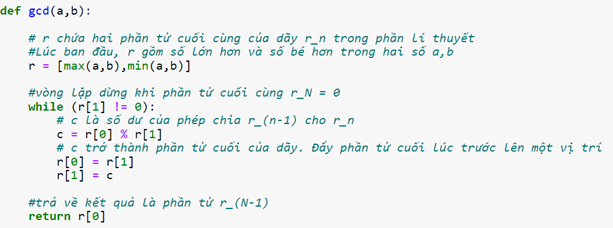
\includegraphics[width=1\linewidth]{2}
		%		\caption{\small\textit{\color{}.}}
		\vspace*{-15pt}
	\end{figure}
	\begin{multicols}{2}
	một tổ hợp tuyến tính của hai phần tử đúng trước nó và do đó cũng là tổ hợp tuyến tính của hai phần tử đầu tiên. Điều này dẫn đến việc ước chung lớn nhất $(r_{N-1})$ mà ta tìm được cũng là một tổ hợp tuyến tính của hai số ban đầu. Đến đây, ta cũng đã chứng minh được phần trước của bổ đề Bézout.
	\vskip 0.1cm
	Ta có thể lập trình một hàm trong Python để tính ước chung lớn nhất sử dụng thuật toán Euclid như trên đây (ý nghĩa của các dòng lệnh được giải thích trong phần comment):
	\vskip 0.1cm
	Khi gọi hàm trên, ta sẽ nhận được kết quả là ước chung lớn nhất của hai số.
	\begin{figure}[H]
		\centering
		\vspace*{-10pt}
		\captionsetup{labelformat= empty, justification=centering}
		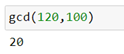
\includegraphics[width=0.4\linewidth]{3}
%		\caption{\small\textit{\color{}.}}
		\vspace*{-15pt}
	\end{figure}
	$\pmb{3.}$ \textbf{\color{hoccungpi}Thuật toán Euclid mở rộng}
	\vskip 0.1cm
	Đến đây thì ta đã giải quyết được vấn đề khi nào bài toán hai can nước có nghiệm. Tuy nhiên, để có thể đưa ra được lời giải cho bài toán, ta cần mở rộng thuật toán Euclid để tính cả các hệ số của tổ hợp tuyến tính biểu diễn ước chung lớn nhất. Với mỗi phần tử $r_n$, ta còn phải tính cả các hệ số $s_n$ và $t_n$ sao cho $r_n=s_n\cdot a+t_n\cdot b$.
	\vskip 0.1cm
	Với hai giá trị đầu của dãy,
	\begin{align*}
		r_0=a=1\cdot a+0\cdot b\\
		r_1=b=0\cdot a+1\cdot b
	\end{align*}
	nên $s_0=1$, $t_0=0$, $s_1=0$, $t_1=1$.
	\vskip 0.1cm
	Đồng thời, do
	\begin{align*}
		r_{n+1}&=r_{n-1}-q_n r_n\\
		&=\left(s_{n\!-\!1}\!\cdot\! a+t_{n-1}\!\cdot\! b\right)-q_n \left(s_n\!\cdot\! a+t_n\!\cdot \!b\right)\\
		&=\left(s_{n-1}-q_n s_n \right)\cdot a+\left(t_{n-1}-q_n t_n \right)\cdot b. 
	\end{align*}
	nên:
	\begin{align*}
		s_{n+1}=s_{n-1}-q_n s_n
		t_{n+1}=t_{n-1}-q_n s_n.
	\end{align*}
	Do ước chung lớn nhất cần tìm là $r_{N-1}$ (khi đã tính ra $r_N=0$), nên ta cũng chỉ cần tính đến $s_{N-1}$ và $t_{N-1}$.
	\vskip 0.1cm
	Ví dụ với $a=48,b=18$ ta có bảng sau:
	\begin{table}[H]
		\vspace*{-5pt}
		\centering
		\captionsetup{labelformat= empty, justification=centering}
		\setlength{\tabcolsep}{8pt}
		\renewcommand{\arraystretch}{1.15}
		\begin{tabular}{|c|c|c|c|c|}
			\hline
			$n$	&$r_n$&	$q_n$&	$s_n$&	$t_n$\\
			\hline
			$0$	&$48$&	&	$1$&	$0$\\
			\hline
			$1$	&$18$&	$2$&	$0$&	$1$\\
			\hline
			$2$&	$12$&	$1$&	$1$&	$-2$\\
			\hline
			$3$&	$6$&	$2$&	$-1$&	$3$\\
			\hline
			$4$&	$0$ & & &\\
			\hline	
		\end{tabular}
		\vspace*{-5pt}
	\end{table}		
	Từ bảng này, ta có ước chung lớn nhất của $48$ và $18$ là $6=-1\cdot 48+3\cdot 18$.
	\vskip 0.1cm
	Đồng thời, kết quả này cũng cho phép ta xác định tổ hợp tuyến tính cho bất kỳ một bội số nào của ước chung lớn nhất. Ví dụ:
	\begin{align*}
		&12=2\cdot 6=-2\cdot 48+6\cdot 18 \\
		&18=3\cdot 6=-3\cdot 48+9\cdot 18 \\
		&\vdots\\
		&72=12\cdot 6=-12\cdot 48+36\cdot 18 \\
		&\vdots
	\end{align*}
	Ta có thể bổ sung vào hàm Python tính ước chung lớn nhất theo thuật toán Euclid để được thuật toán Euclid mở rộng như trong hình dưới:
	\begin{figure}[H]
		\centering
		\vspace*{-5pt}
		\captionsetup{labelformat= empty, justification=centering}
		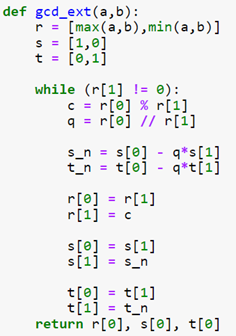
\includegraphics[width=0.75\linewidth]{4}
%		\caption{\small\textit{\color{}.}}
		\vspace*{-10pt}
	\end{figure}
	Ở đây, ta đã thêm hai danh sách $s$ và $t$ để lưu hai phần tử cuối của các dãy $s_n$ và $t_n$ như trong phần lý thuyết. Các giá trị của hai dãy này được tính theo công thức của chúng. Cần lưu ý rằng toán tử // là phép chia cho ra thương số của phép chia có dư. Việc đẩy các giá trị mới vào các danh sách $s,t$ cũng tương tự như với $r$.
	\vskip 0.1cm
	Hàm trên trả ra một bộ ba số gồm ước chung lớn nhất và các tham số s,t gắn với nó.
	\begin{figure}[H]
		\centering
		\vspace*{-5pt}
		\captionsetup{labelformat= empty, justification=centering}
		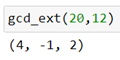
\includegraphics[width=0.4\linewidth]{5}
		%		\caption{\small\textit{\color{}.}}
		\vspace*{-10pt}
	\end{figure}
	Ví dụ với $a=20,b=12,$ ta có: $4=(-1)\cdot 20+2\cdot 12$
	\vskip 0.1cm
	Tổ hợp tuyến tính cho lượng nước cần đong $k$ có thể cho ta cách giải của bài toán hai can nước. Do $k$ sẽ nhỏ hơn giá trị lớn nhất trong hai số $a,b$ nên sẽ luôn có một trong hai hệ số của tổ hợp tuyến tính nhận giá trị âm và hệ số còn lại nhận giá trị dương. Can ứng với hệ số dương là can đầu vào (đổ từ bể vào can) còn can ứng với hệ số âm là can đầu ra (đổ từ can vào lại bể).
	\vskip 0.1cm
	Cách đong của ta được tiến hành như sau:
	\vskip 0.05cm
	$\bullet$ Nếu can đầu vào rỗng thì đổ đầy nó.
	\vskip 0.05cm
	$\bullet$ Nếu can đầu vào không rỗng thì đổ sang can đầu ra cho đến khi nó đầy hoặc can đầu vào hết nước.
	\vskip 0.05cm
	$\bullet$ Nếu can đầu ra đầy thì đổ hết nước bên trong trở lại bể.
	\vskip 0.05cm
	Giá trị tuyệt đối của các hệ số trong tổ hợp tuyến tính sẽ cho ta biết số lần phải đổ đầy can đầu vào cũng như số lần đổ hết nước ở can đầu ra trở lại bể.
	\vskip 0.05cm
	Ta hãy xét trường hợp lượng nước cần đong bằng với ước chung lớn nhất của dung tích hai can. Ví dụ, đong $1$ lít từ hai can $5$ lít và $8$ lít. Thuật toán Euclid cho ta $1=2\cdot 8-3\cdot 5$. Ta có can $8$ lít là can đầu vào còn can $5$ lít là can đầu ra.
	\vskip 0.05cm
	Quy trình đong như sau:
	\begin{table}[H]
		\vspace*{-5pt}
		\centering
		\captionsetup{labelformat= empty, justification=centering}
		\setlength{\tabcolsep}{7pt}
		\renewcommand{\arraystretch}{1.1}
		\begin{tabular}{|l|c|c|}
			\hline
			Bước làm&	Can $8$ lít&	Can $5$ lít\\
			\hline
			Đổ đầy can $8$ lít&	$8$&	$0$\\
			\hline
			Đổ sang can $5$ lít&	$3$&	$5$\\
			\hline
			Đổ hết can $5$ lít&	$3$&	$0$\\
			\hline
			Đổ sang can $5$ lít&	$0$&	$3$\\
			\hline
			Đổ đầy can $8$ lít&	$8$&	$3$\\
			\hline
			Đổ sang can $5$ lít&	$6$&	$5$\\
			\hline
			Đổ hết can $5$ lít&	$6$&	$0$\\
			\hline
			Đổ sang can $5$ lít&	$1$&	$5$\\
			\hline
			Đổ hết can $5$ lít&	$1$	&$0$\\
			\hline
		\end{tabular}
		\vspace*{-10pt}
	\end{table}
	Trong lời giải trên, ta đã đổ đầy can $8$ lít $2$ lần và đổ hết can $5$ lít $3$ lần đúng như các hệ số tương ứng. Nói cách khác, biểu thức theo dạng bổ đề Bézout cho ta một biểu diễn của lời giải bằng một tổ hợp tuyến tính của $a$ và $b$.
	\vskip 0.1cm
	Vậy nếu ta muốn đong một lượng lớn hơn thì sao? Giả sử thay vì $1$ lít, ta muốn đong $2$ lít từ các can trên thì ta sử dụng $2=2\cdot 1=4\cdot 8-6\cdot 5$ và làm tương tự.
	\vskip 0.1cm
	\textbf{\color{hoccungpi}Bài tập}
	\vskip 0.1cm
	$a)$ Hãy lập bảng như trên cho trường hợp đong $2$ lít từ hai can $8$ lít và $5$ lít.
	\vskip 0.1cm
	$b)$ Làm tương tự cho trường hợp muốn đong $4$ lít.
	\vskip 0.1cm
	$\pmb{4.}$ \textbf{\color{hoccungpi}Phương trình Diophantine tuyến tính}
	\vskip 0.1cm
	Quay lại bảng cho trường hợp $1$ lít, ta nhận thấy chỉ cần ngay trong lượt đong đầu tiên, ta đã thu được $3$ lít và lượng nước 6 lít cũng xuất hiện luôn ở cuối lượt đong thứ hai. Trong khi đó, nếu ta giải theo dạng bội của ước chung lớn nhất như cách làm ở phần trước thì số lượt đong sẽ nhiều hơn nhiều ($3=6\cdot 8-9\cdot 5$; $6=12\cdot 8-18\cdot 5$).
	\vskip 0.1cm
	Để giải thích việc này, ta hãy nhìn lại phương trình cần giải cho trường hợp $3$ lít:
	\begin{align*}
		8x+5y=3.	\tag{$4$}
	\end{align*}
	Phương trình trên thuộc dạng phương trình Diophantine tuyến tính: 
	\begin{align*}
		ax+by=c.
	\end{align*}
	Trong các phương trình dạng này, người ta quan tâm đến các nghiệm x,y là số nguyên. Một nghiệm của phương trình đã được cung cấp bằng cách lấy bội của kết quả từ thuật toán Euclid cho hai số $8$ và $5$ như ở trên:
	\begin{align*}
		8\cdot 6+5\cdot (-9)=3
	\end{align*}
	Các phương trình Diophantine được đặt tên theo nhà toán học Hy Lạp, Diophantus. Ông sống ở Alexandria vào khoảng thế kỷ thứ $3$ sau Công nguyên. Các phương trình mà ông nghiên cứu chỉ cho phép các nghiệm là số nguyên. Ngày nay, chúng vẫn là đề tài của nhiều nghiên cứu toán học hiện đại.
	\vskip 0.1cm
	Chúng ta hãy thử tìm xem còn có nghiệm nào khác của phương trình này không. Không mất tính tổng quát, giả sử phương trình còn có nghiệm $x=6+u$, $y=-9+v$ với $u,v$ là các số nguyên. Thay vào phương trình ban đầu ta được:
	\begin{align*}
		8\cdot (6+u)+5\cdot (-9+v)&=3\\
		(8u+5v)+(8\cdot 6-5\cdot 9)&=3\\
		8u+5v&=0		\tag{$5$}
	\end{align*}
	Phương trình ($5$) là phương trình Diophantine thuần nhất (vế phải bằng $0$) tương ứng với phương trình ($4$). Viết lại ($5$) dưới dạng $8u=-5v$, ta thấy vì $8$ và $5$ là hai số nguyên tố cùng nhau nên $u$ phải chia hết cho $5$. Đặt $u=5p$, ta được $v=-8p$ với $p$ là số nguyên. Do $p$ có thể nhận vô số giá trị, phương trình thuần nhất của ta có vô số nghiệm. 
	\vskip 0.1cm
	Phương trình ($4$) cũng sẽ có vô số nghiệm xác định bởi: 
	\begin{align*}
		x&=6+5p\\
		y&=-9-8p.
	\end{align*}
	Chú ý rằng phương trình ($4$) có nghiệm là do vế phải là một bội của ước chung lớn nhất của hai số $8$ và $5$, theo bổ đề Bézout. Trong trường hợp phương trình thuần nhất có hai hệ số không nguyên tố cùng nhau, ta cần chia cả hai vế cho ước chung lớn nhất của hai hệ số rồi tiến hành giải tương tự như trên.
	\vskip 0.1cm
	\textbf{\color{hoccungpi}Bài tập}
	\vskip 0.1cm
	Hãy giải các phương trình nghiệm nguyên sau:
	\vskip 0.1cm
	$a)$ $6x+9y=24$
	\vskip 0.1cm
	$b)$ $4x+12y=44$
	\vskip 0.1cm
	Từ họ nghiệm cho phương trình ($4$), ta hãy nhìn lại trường hợp đong $3$ lít từ hai can $8$ lít và $5$ lít. Ta sẽ có vô số nghiệm để chọn bằng cách thay đổi $p$. Giả sử ta muốn số lần đổ đầy can $8$ lít là ít nhất. Khi đó $p=-1$, ta được nghiệm $x=1$; $y=-1$ hay $8-5=3$ ứng với việc đổ đầy can $8$ lít rồi rót trực tiếp từ can $8$ lít sang can $5$ lít. Trong trường hợp muốn chọn can $5$ lít làm can đầu vào và can $8$ lít làm can đầu ra, ta cần cho y nhận giá trị dương. Giá trị dương nhỏ nhất của $y$ ứng với $p=-2$ hay $x=-4$; $y=7$. Độc giả có thể thử lập bảng các thao tác cho trường hợp này.
	\vskip 0.1cm
	Đến đây, ta đã có thể liệt kê tất cả các lời giải của bài toán hai cái can bằng cách sử dụng thuật toán Euclid mở rộng và giải phương trình Diophantine. Tiếp theo, chúng ta sẽ tìm hiểu một số biến thể của bài toán hai cái can.
	\vskip 0.1cm
	$\pmb{5.}$ \textbf{\color{hoccungpi}Một số biến thể của bài toán hai cái can}
	\vskip 0.1cm 
	Ta hãy xét một bài toán khác cũng với hai cái can. 
	\vskip 0.1cm
	Giả sử có hai bể nước. Bể $1$ đầy nước còn bể $2$ không có nước. Với hai can có dung tích $a$ và $b$ lít, hãy đong $k$ lít từ bể $1$ vào bể $2$.
	\vskip 0.1cm
	Bài toán này cũng quy về giải phương trình Diophantine tuyến tính:
	\begin{align*}
		ax+by=k.
	\end{align*}
	Vẫn theo bổ đề Bézout, bài toán có nghiệm khi $k$ là một bội của ước chung lớn nhất $d$ của $a$ và $b$.
	\vskip 0.1cm
	Khi viết lời giải, ta cần không sử dụng thao tác đong từ can nọ sang can kia mà chỉ cần $s$ lần đong đầy can $a$ và $t$ lần đong đầy can $b$ từ bể $1$ đổ sang bể $2$. Các trường hợp hệ số $s$ hoặc $t$ âm ứng với việc đổ ngược lại từ bể $2$ sang bể $1$.
	\vskip 0.1cm
	Vẫn xét trường hợp hai can $8$ lít và $5$ lít nhưng phải đong $36$ lít sang bể $2$. Từ thuật toán Euclid mở rộng, $8\cdot 2+5\cdot (-3)=1$ nên $8\cdot 72+5\cdot (-108)=36$. Phương trình Diophantine $8x+5y=36$ sẽ có họ nghiệm 
	\begin{align*}
		&x=72+5p\\
		&y=-108-8p
	\end{align*}
	với $p$ là số nguyên.
	\vskip 0.1cm
	Ta hãy nhìn nhận các nghiệm từ khía cạnh thực tế. Nếu cả $x$ và $y$ đều dương thì ta chỉ cần vận chuyển đúng $36$ lít. Nếu có một trong hai giá trị $x$ và $y$ âm thì ta phải đổ nhiều hơn $36$ lít vào bể $2$ và đổ lại phần thừa ra vào bể $1$. Khi đó tổng lượng nước phải vận chuyển sẽ nhiều hơn $36$ lít. Do đó, nếu muốn tiết kiệm công sức, ta chỉ nên xét các nghiệm $x$, $y$ dương. 
	\vskip 0.1cm
	Giải hệ
	\begin{align*}
		72+5p \ge 0\\
		-108-8p\ge 0
	\end{align*}
	ta thấy chỉ có $p=-14$ thỏa mãn. Khi đó $x=2$; $y=4$. Ta cần đổ $2$ lần can $8$ lít và $4$ lần can $5$ lít từ bể $1$ vào bể $2$. Với các giá trị $a,b,k$ khác, có thể có nhiều hơn một giá trị $p$ để cho $x,y$ dương.
	\vskip 0.1cm
	Mặt khác, nếu khoảng cách giữa hai bể là tương đối xa, thì tổng số lượt đi lại có thể quan trọng hơn tổng lượng nước phải vận chuyển do mỗi một lượt ta chỉ có thể vận chuyển một can (giả sử chỉ có một người thao tác). Xét ví dụ $a=9$, $b=2$, $k=34$. Các nghiệm $x,y$ dương của trường hợp này bao gồm: $9\cdot 0+2\cdot 17=34$ và $9\cdot 2+2\cdot 16=34$.
	\vskip 0.1cm
	Trong khi đó, nếu ta chấp nhận nghiệm âm, số lượt phải đi ít nhất khi một trong hai giá trị $x,y$ âm sẽ ứng với nghiệm $9\cdot 4-2\cdot 1=34$. Tuy ta phải vận chuyển tổng cộng $38$ lít nước trong trường hợp này, số lượt di chuyển chỉ có $5$ lượt, ít hơn nhiều so với hai nghiệm nêu trên.
	\vskip 0.1cm
	\textbf{\color{hoccungpi}Bài tập}
	\vskip 0.1cm
	Hãy giải các bài toán sau và tìm phương án với số lần di chuyển hai can ít nhất:
	\vskip 0.1cm
	$a)$ Dùng hai can $6$ lít và $11$ lít đong $51$ lít vào bể $2$.
	\vskip 0.1cm
	$b)$ Dùng hai can $7$ lít và $10$ lít đong $43$ lít vào bể $2$.
	\vskip 0.1cm
	Ta còn có thể mở rộng bài toán ra trường hợp có nhiều can. Để cho đơn giản, ta hãy xét trường hợp sử dụng $3$ can dung tích $a,b,c$ để đong $k$ lít nước từ bể $1$ sang bể $2$, phương trình Diophantine tuyến tính của ta có dạng:
	\begin{align*}
		ax+by+cz=k.
	\end{align*}
	Về điều kiện tồn tại nghiệm của phương trình này, ta cần mở rộng định lý Bézout cho trường hợp $3$ số.
	\vskip 0.1cm
	Gọi $d$ là ước chung lớn nhất của $a$ và $b$. Ta sử dụng thuật toán Euclid mở rộng hai lần: 
	\vskip 0.1cm
	$\bullet$ Biểu diễn $d$ theo $a$ và $b$.
	\vskip 0.1cm 
	$\bullet$ Biểu diễn ước chung lớn nhất $g$ của theo $c$ và $d$ theo hai số này. Hãy nhớ rằng ước chung lớn nhất $g$ của $c$ và $d$ cũng là ước chung lớn nhất của ba số $a,b,c$.
	\vskip 0.1cm
	Thế biểu diễn của $d$ theo $a,b$ vào biểu diễn của $g$ theo $c,d$ để cho ra biểu diễn cuối cùng của $g$ theo $a,b,c$.
	\vskip 0.1cm 
	Theo cách này, ta luôn có thể tìm được biểu diễn của ước chung lớn nhất của ba số theo một tổ hợp tuyến tính của chúng.
	\vskip 0.1cm
	\textbf{\color{hoccungpi}Bài tập}
	\vskip 0.1cm
	$a)$ Chứng minh rằng $\text{ƯCLN}(a,b,c) = \text{ƯCLN}(\text{ƯCLN}(a,b), c)$
	\vskip 0.1cm
	$b)$ Dùng nhận định trên để tìm ước chung lớn nhất của $48$, $72$ và $81$.
	\vskip 0.1cm
	Điều kiện tồn tại nghiệm vẫn là $k$ phải chia hết hết cho ước chung của cả ba số $a,b,c$. Cách chứng minh tương tự như trường hợp bổ đề Bézout cho hai số.
	\vskip 0.1cm
	Để giải phương trình Diophantine cho $3$ số, ta cần tiến hành theo hai bước, mỗi bước giải một phương trình Diophantine cho $2$ số. Cách làm được minh họa cho ví dụ sau:
	\begin{align*}
		8x+6y+7z=20. \tag{$6$}
	\end{align*}
	Trước hết, vì ước chung lớn nhất của $8$ và $6$ là $2$ nên $8x+6y$ sẽ luôn chia hết cho $2$ theo bổ đề Bézout. Do đó, ta đặt $8x+6y=2u$. Thế vào ($6$), ta được:
	\begin{align*}
		2u+7z=20.
	\end{align*}
	Thuật toán Euclid mở rộng cho ta $1=2\cdot (-3)+7\cdot 1$. Do đó $20=2\cdot (-60)+7\cdot 20$. Kết hợp với phương trình thuần nhất ta được:
	\begin{align*}
		&u=-60+7p\\
		&z=20-2p
	\end{align*}
	với $p$ là số nguyên.
	\vskip 0.1cm
	Ta có:
	\begin{align*}
		8x+6y=2u=-120+14p.
	\end{align*}
	Thuật toán Euclid mở rộng cho ta: $2=8\cdot 1+6\cdot (-1)$. Do đó 
	\begin{align*}
		-120+14p&=2\!\cdot\! (\!-\!60\!+\!7p)\\
		&=8\!\cdot\! (\!-\!60\!+\!7p)\!+\!6\!\cdot\! (60\!-\!7p).
	\end{align*}
	Kết hợp với phương trình thuần nhất, ta được:
	\begin{align*}
		x&=-60+7p+6q\\
		y&=60-7p-8q
	\end{align*}
	với $q$ là số nguyên.
	\vskip 0.1cm
	Nghiệm cuối cùng của bài toán có dạng:
	\begin{align*}
		x&=-60+7p+6q\\
		y&=60-7p-8q\\
		z&=20-2p
	\end{align*}
	với $p,q \in \mathbb{Z}$.
	\vskip 0.1cm
	Đến đây ta đã hoàn toàn có thể giải được bài toán cho trường hợp $3$ cái can.
	\vskip 0.1cm
	Cho trường hợp $n>3$ cái can, các chứng minh lý thuyết cùng việc giải phương trình cũng tương tự trường hợp $3$ cái can. Chú ý rằng khi giải phương trình Diophantine tuyến tính cho $n$ ẩn số, ta cần thế từng bước, hai ẩn số một lần.
	\vskip 0.1cm
	\textbf{\color{hoccungpi}Bài tập}
	\vskip 0.1cm
	Hãy giải phương trình nghiệm nguyên sau:
	\begin{align*}
		5x+9y+12z=136.
	\end{align*}
	$\pmb{6.}$ \textbf{\color{hoccungpi}Kết luận}
	\vskip 0.1cm
	Bài toán hai cái can là một bài toán quen thuộc ở bậc tiểu học nhưng đồng thời cũng có những liên hệ thú vị đến các kiến thức phép chia hết và số nguyên tố ở lớp $6$. Tác giả hy vọng bài viết có thể giúp cho việc giảng dạy về lý thuyết số ở bậc trung học cơ sở cho những học sinh muốn tìm hiểu sâu hơn về toán học trở nên dễ dàng hơn.
	\vskip 0.1cm
	\textbf{\color{hoccungpi}Tài liệu tham khảo}
	\vskip 0.1cm
	[$1$] Apostol, T.M. ($2010$). \textit{Introduction to analytic number theory}. New York: Springer.
	\vskip 0.1cm
	[$2$] Titu Andreescu, D Andrica and Ion Cucurezeanu ($2010$). \textit{An introduction to diophantine equations : a problem-based approach}. New York: Birkhäuser.
\end{multicols}